\section{Calibration Sample Audit}

\noindent\begin{minipage}{\columnwidth}
{\centering
  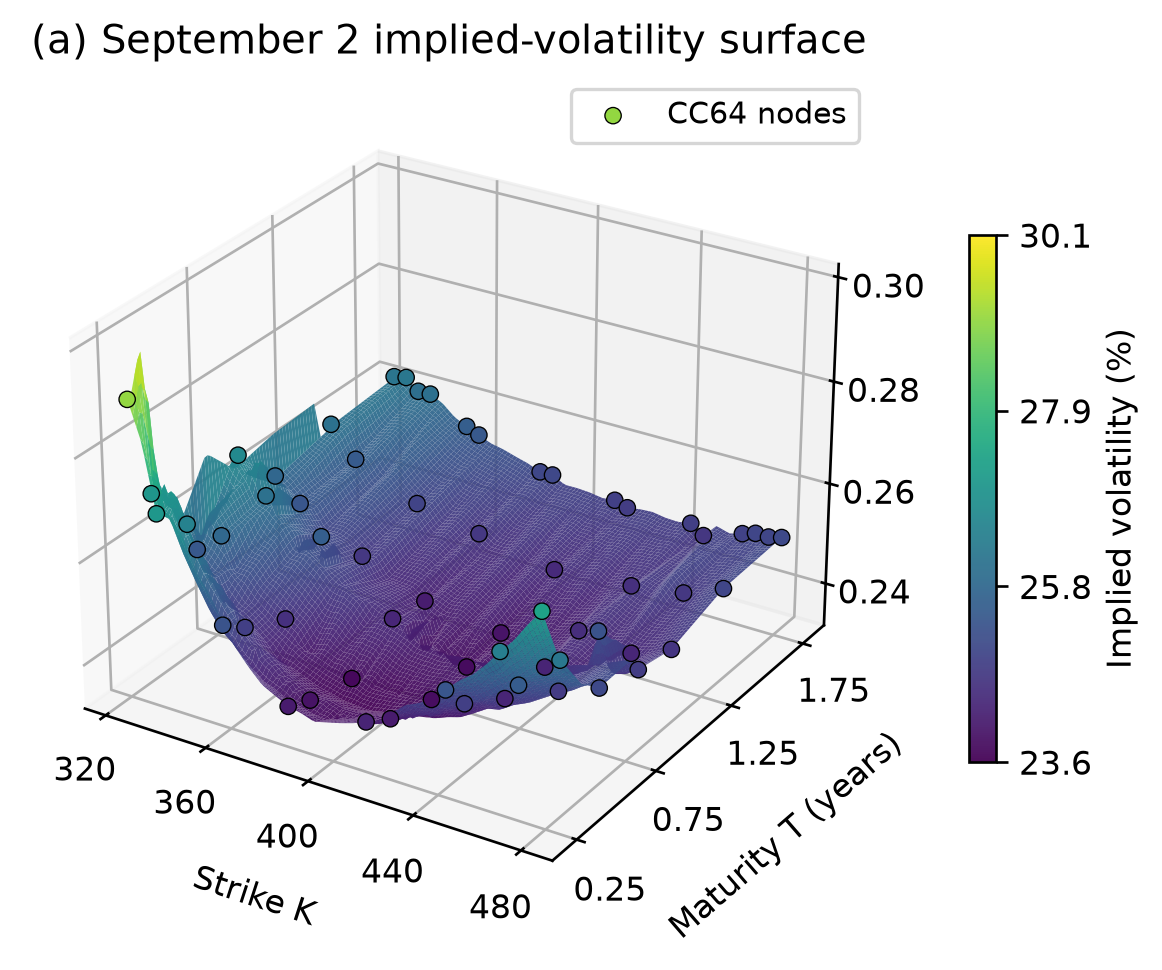
\includegraphics[width=\columnwidth]{../img/publication/6c5ba226b4a1f62f_sampling_surface_current.png}
  \captionof{figure}{(a) GLD implied-volatility surface, 2 September 2026, with CC64 nodes. Interpolation is used for display only.}
  \label{fig:chebyshev_audit}
\par}
\end{minipage}\par

\noindent\begin{minipage}{\columnwidth}
{\centering
  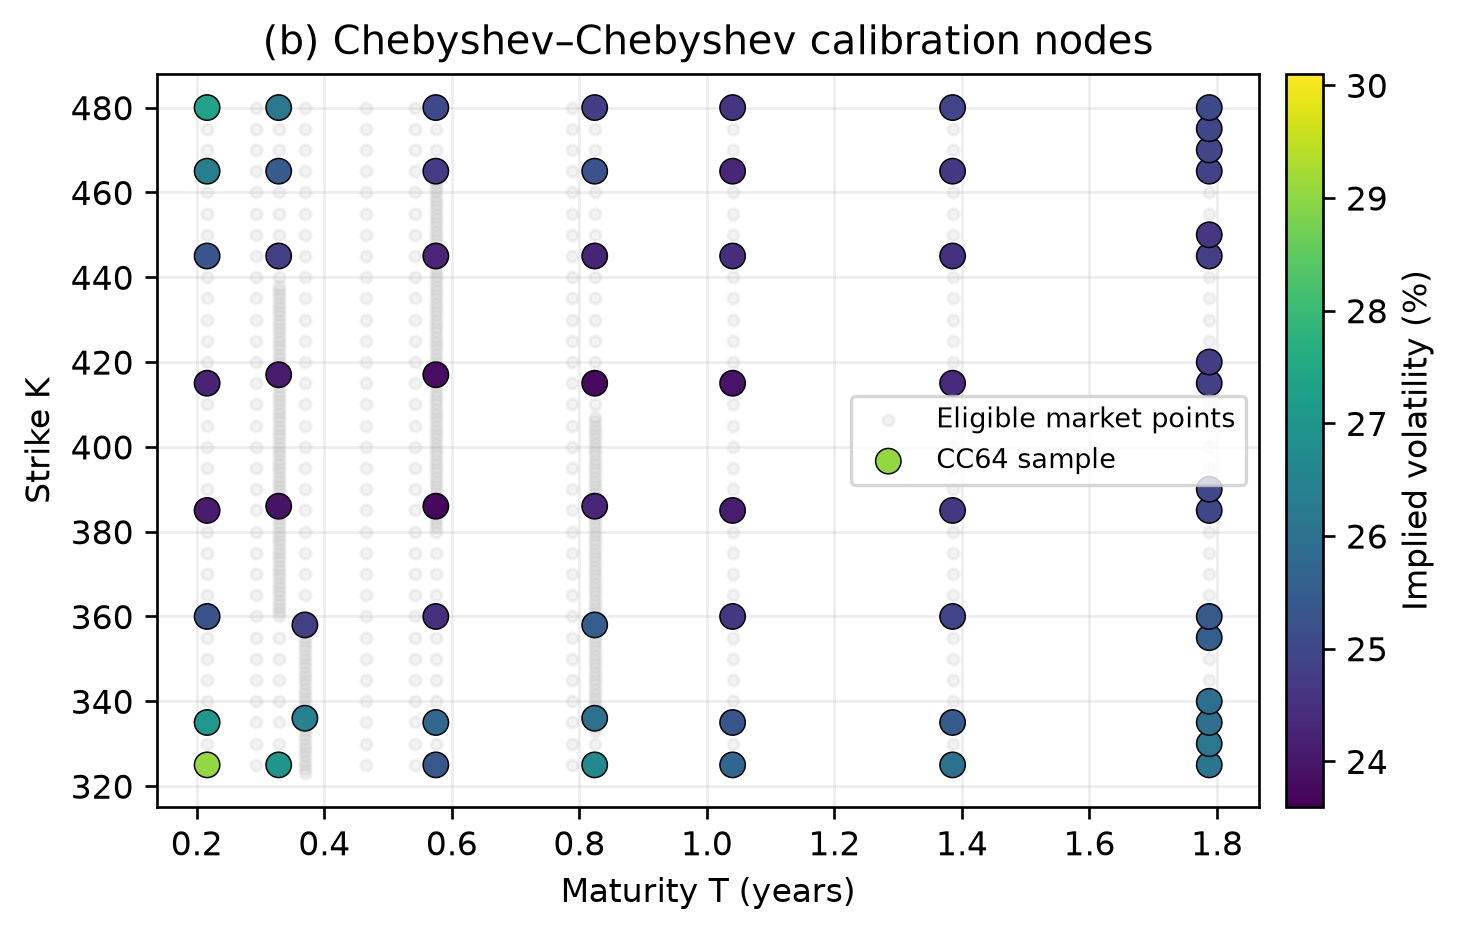
\includegraphics[width=0.95\columnwidth]{../img/publication/498fa63273eb3ac5_sampling_nodes.png}
  \captionof*{figure}{\textbf{Figure~\ref{fig:chebyshev_audit} (continued).} (b) The 64 actual contracts selected from 605 eligible calls across 12 expiries and 146 strikes.}
\par}
\end{minipage}\par

\subsection{Why structured sampling is retained}
The option surface is irregular in strike and maturity. Team 8 therefore passes a fixed $8\times8$ Chebyshev--Chebyshev subset to the optimizer rather than allowing densely listed regions to dominate the loss. Every target is mapped to the nearest still-unused actual option: the 64-point calibration set contains no synthetic contracts. The figure audits the same 2 September parameter snapshot used by the refreshed valuation.

\begin{methodbox}[Evidence status]
The residual maps, the parameters and the valuation paths come from one recalibration of the 2 September sample with $q=0.40\%$, dated 24 October 2026. The Treasury curve and the gold spot anchor are dated 2 September as well.
\end{methodbox}

\subsection{What the residual maps add}
The residual heatmaps show where each specification systematically over- or under-prices the observed implied-volatility surface. Black--Scholes leaves the strongest smile and term-structure pattern. Bates is refined from the nested Heston point and Bates--Hawkes from the nested Bates point, so each richer model fits at least as well as the model it contains (Table~\ref{tab:iv_rmse}). All maps use one colour scale; calibration fit does not establish economic superiority.

\noindent\begin{minipage}{\columnwidth}
{\centering
  \includegraphics[width=0.95\linewidth]{\FigBlackScholesResidualHeatmap}
  \par\vspace{1pt}{\footnotesize\textbf{(a)} Black--Scholes\par}
  \vspace{3pt}
  \includegraphics[width=0.95\linewidth]{\FigHestonResidualHeatmap}
  \par\vspace{1pt}{\footnotesize\textbf{(b)} Heston\par}
  \captionof{figure}{Implied-volatility residual maps for the common 2 September CC64 sample with $q=0.40\%$. Blue denotes model IV above market IV and red denotes model IV below market.}
  \label{fig:residual_maps}
\par}
\end{minipage}\par

\vspace{4pt}
\noindent\begin{minipage}{\columnwidth}
{\centering
  \includegraphics[width=0.95\linewidth]{\FigBatesResidualHeatmap}
  \par\vspace{1pt}{\footnotesize\textbf{(c)} Bates--Poisson\par}
  \vspace{3pt}
  \includegraphics[width=0.95\linewidth]{\FigBatesHawkesResidualHeatmap}
  \par\vspace{1pt}{\footnotesize\textbf{(d)} Full Bates--Hawkes\par}
  \captionof*{figure}{\textbf{Figure~\ref{fig:residual_maps} (continued).} Bates--Poisson and Full Bates--Hawkes residual maps; all colourbars share the same residual range.}
\par}
\end{minipage}\par

\begin{table}[H]
\centering
\caption{Current-surface IV calibration RMSE (bp). The 7 September column used $q=0$; the IV targets differ, so the columns are not a like-for-like fit comparison.}
\label{tab:iv_rmse}
\begin{tabular}{@{}lrr@{}}
\toprule
Model & $q=0.40\%$ & 7 Sep, $q=0$ \\
\midrule
Black--Scholes & \CalBSIVRMSE & \CalBSIVRMSELegacy \\
Heston & \CalHIVRMSE & \CalHIVRMSELegacy \\
Bates--Poisson & \CalBIVRMSE & \CalBIVRMSELegacy \\
Full Bates--Hawkes & \CalWIVRMSE & \CalWIVRMSELegacy \\
\bottomrule
\end{tabular}
\end{table}

\subsection{What the fit can and cannot identify}
With the fee as carry the fit deteriorates: the Heston price RMSE rises from USD~\CarryPriceRMSEZero{} to \CarryPriceRMSEFee{}, and the loss increases in every moneyness bucket. The calls therefore price a higher carry than Treasury rates less the fee. Call-only surfaces cannot separate that carry from skew, so a fitted carry would not be a forward; the futures-implied fee is used instead, and identifying the forward would need puts or box-spread rates.

\begin{methodbox}[Calibration fragility]
The Feller condition is imposed as a hard constraint and binds at the optimum for Bates and Bates--Hawkes; without it the Heston loss falls by \FellerRelaxedLossRatio\%. The Heston loss changes by less than 3\% for $\kappa$ between \KappaFlatLow{} and \KappaFlatHigh, so mean reversion is weakly identified. With $q=0.40\%$ the Bates jump intensity is \BatesLambda{} a year rather than zero, but jump and Hawkes parameters rest on 64 calls and are not individually identified. Bates--Hawkes branching is \HawkesBranching{} with a kernel half-life of \HawkesHalfLifeDays{} days.
\end{methodbox}
